\chapter{Background Research: Recommender Systems}

This section introduces the fundamental concepts of recommender and machine learning systems. Then, it discusses different techniques as well as algorithms. Finally, existing solutions are evaluated.

\section{Definition}

Recommendations are neither a new idea nor limited to the digital age. \citet{ricci11} write that traditional recommendations can be observed in various scenarios, such as a peer's recommendation when buying a book or reviews when choosing a movie. The authority of the recommender has an important role in the acceptance of the recommendation. A renowned film critic may appear more credible than a random colleague. When it comes to car parts, a mechanist may be a good candidate to ask. However the authority is not only limited to expertise -- in fact we tend to rely more on recommendations which put our personal experiences and preferences into account. A previous companion for a wonderful trip can certainly have a better authority than a travel agent.

As mentioned in the introduction, with the growth of the Internet, the amount of information available on the Web increased rapidly. Especially major e-commerce Web sites were extending their range of products and services. Although a wider and varied range of items is initially good for the user, users found it more and more difficult to find the appropriate items or make the right choices. Web sites have deployed different type of solutions -- such as search engines and more user friendly interfaces -- to cope with this problem.

Another approach are recommender systems which basically provides a bespoke collection of items with the intention to highlight relevant items to a user. Depending on the recommending technique various data sources are taken into account being the user's context or previous interactions. It is a continuous learning process. The more it learns, the more accurate the recommendations will become. The user's behaviour on given recommendations are further a powerful learning source for the system -- e.g. if the user tends to accept some recommendations over others -- to tweak the recommendations. Most recommender systems concentrate on guiding the user towards new, unexperienced items \cite{ricci11}.

Recommender systems are autonomous and utilize machine learning principles which is a branch of artificial intelligence (AI). Latter is defined by \citeasnoun{mccarthy07} as \textit{'the science and engineering of making intelligent machines, especially intelligent computer programs'}. In that sense, machine learning enables computers to learn from data passed through it to be able to make predictions about future data. In other words the learning machine tries to generalize. It is based on the assumption that almost all data includes \textit{patterns} -- any repeating regularity that describes the \textit{model} the learning machine is concerned about. This allows learning machines to generalise \cite{segaran07}.

\section{Adoption}

\citeasnoun{ricci11} also note that research on recommender systems is relatively new compared to other classical information retrieval methods like databases and search engines. However it is gaining attention due to various reasons. First of all e-commerce companies including Amazon, YouTube and Netflix invest a lot in recommender systems. As trendsetters and pioneers for other institutions they build a demand for further research and development. Dedicated conferences and academic courses as well as its adaption in several academic journals are indicators of recognition of this research area.

With regard to beforementioned adoption in e-commerce I will illustrate the usage of sophisticated recommender systems in two examples.

\subsection{Netflix}

\begin{figure}[ht]
    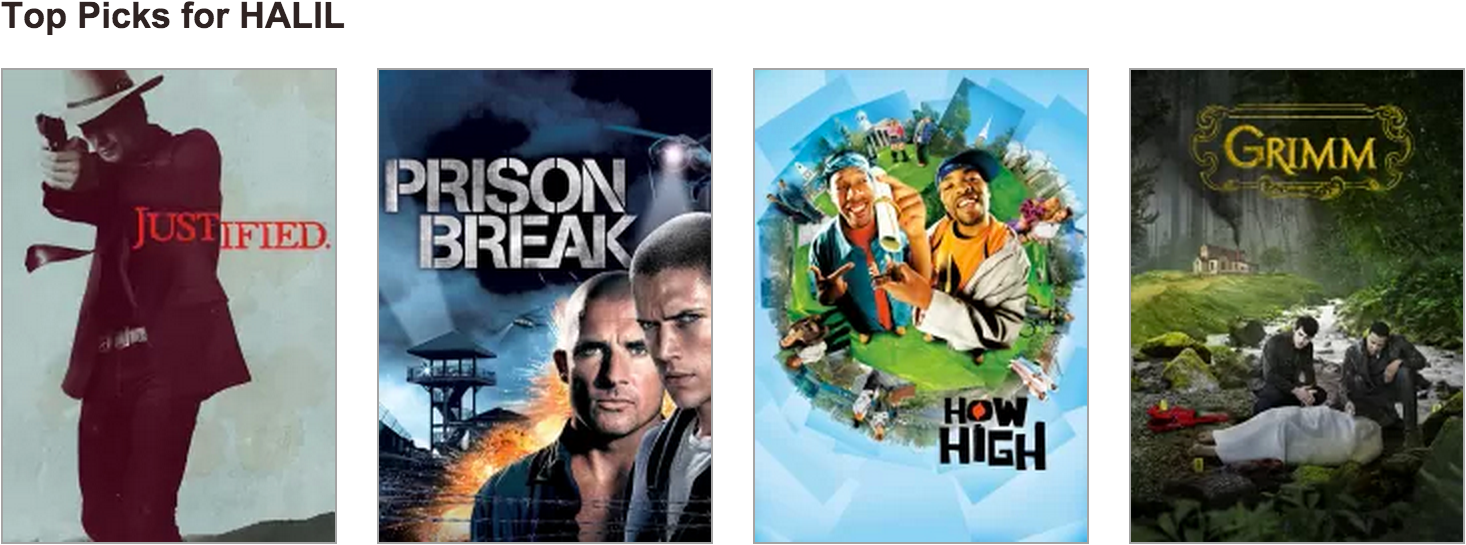
\includegraphics[width=\textwidth,center]{background/adoption/netflix.png}
    \caption{Netflix Recommendations}
    \label{fig:netflix}
\end{figure}

Netflix offers their on-demand video streaming with a simplified user interface across all platforms including smartphones and tablets. There is only limited functionality to navigate through their items. It rather focuses on ranked lists around a topic or genre. Once subscribers start using their service, the recommender system of Netflix on one hand builds new, personalised lists in relation to that item. On the other hand it updates existing lists with that learning.

Their recommender system is such a fundamental part of their business model that they launched a competition called Netflix Prize and called expert teams to propose a more accurate algorithm. They eventually awarded a million dollar to best scoring team \cite{netflix09}.

\subsection{Amazon}

\begin{figure}[ht]
    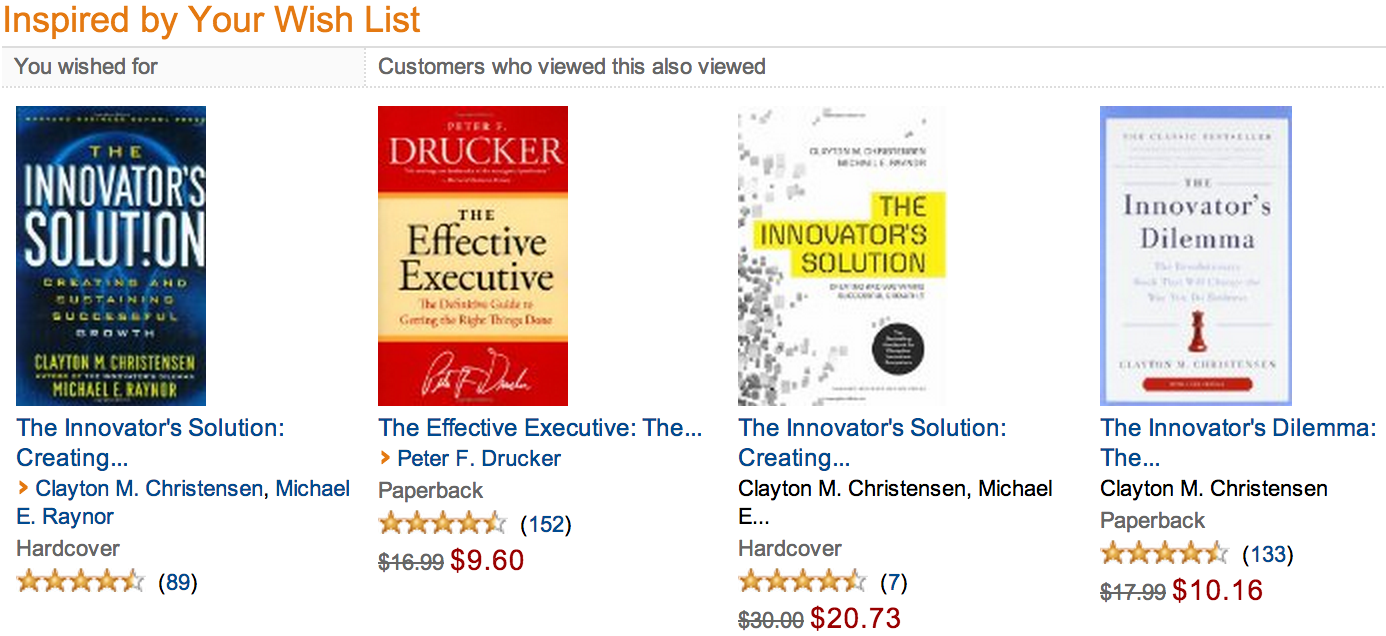
\includegraphics[width=\textwidth,center]{background/adoption/amazon.png}
    \caption{Amazon Recommendations}
    \label{fig:amazon}
\end{figure}

The online retailer Amazon relies on recommender systems throughout their e-commerce platform. They are not limited to the website but are in fact also used in their email campaigns. Amazon inventend \textit{item-based collaborative filtering} which surprisingly focuses on items rather than users and is discussed in detail in section \ref{bg-tech-itembased} \cite{linden03}. The user's collaboration is taken into account to put items into relation.

Moreover Amazon is an examplary user of \textit{automated merchandising} to which I could not find any coverage in literature, although it is an important area for e-commerce companies. Recommender systems are observing the behaviour of the customer on the item collection to predict individual recommendations. However this behaviour can also be used to build objective relations between items such as categorisation and cross-selling (offer additional items to increase basket value). Given that Amazon has more than 200 million products at the time of writing, merchandising the whole catalog manually is almost impossible.

\section{Techniques}

\subsection{Collaborative Filtering}
\label{bg-tech-collaborative}
\label{bg-tech-itembased}

\subsection{Content-Based Filtering}
\subsection{Hybrids}

\section{Algorithms}

\subsection{Pearson Correlation Coefficient}
\subsection{Tanimoto Coefficient}

\section{Evaluation of Existing Solutions}

% apache mahout